\section{Différents phénomènes régis par la même équation}
\subsection{Onde dans une corde}
\lien{https://www.youtube.com/watch?v=jV1Tp_tM2Ts&t=37s}
Les cordes peuvent être le siège d'ondes transversales.

La corde est un milieu unidimensionnel. Une seule direction de propagation est possible.

\schema{Corde}{4cm}

\formule{Équation de propagation}
[\begin{itemize}
    \item La corde est infiniment flexible et inextensible.
    \item Les déplacements sont faibles et transverses.
    \item Les effets de la gravité sont négligés.
    \item Les frottements sont négligés.
\end{itemize}]
{
    $$\frac{\partial^2 y}{\partial x^2}-\frac{1}{c^2}\frac{\partial^2y}{\partial t^2}=0$$
}
[
    \begin{itemize}
        \item $y(x,t)$ la hauteur de la corde à l'abscisse $x$ et à l'instant $t$ (en \unit{m})
        \item $c=\sqrt{\frac{T}{\mu}}$ la célérité de l'onde (en \unit{m.s^{-1}})
        \item $T$ la tension dans la corde (en \unit{N})
        \item $\mu$ la masse linéique de la corde (en \unit{kg.m^{-1}})
    \end{itemize}
][o][o]

\colle{Établir l'équation aux dérivées partielles vérifiée par une onde dans une corde en précisant les hypothèses et approximations effectuées.}
\flashcard{Équation de d'Alembert}{$$\Delta y-\frac{1}{c^2}\frac{\partial^2y}{\partial t^2}=0$$ (ou $$\frac{\partial^2y}{\partial x^2}-\frac{1}{c^2}\frac{\partial^2y}{\partial t^2}=0$$ en 1D)}

Cette équation aux dérivées partielles s'appelle \textbf{équation de d'Alembert}.

\subsection{Ondes dans un cable coaxial}
Un cable coaxial est constitué de deux conducteurs concentriques (l'âme et la gaine) séparés par un isolant. Le cable coaxial est un milieu unidimensionnel.

\begin{figure}[!ht]
    \centering
    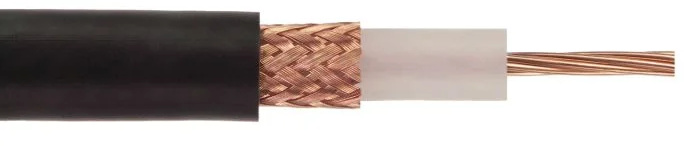
\includegraphics[width=7cm]{images/coaxial.jpg}
    \caption{Photographie d'un cable coaxial.}
\end{figure}

\schema{Cable coaxial}{3cm}

\exemple{Les cables d'antennes (satellite, TNT, wifi, ...) sont souvent des cables coaxiaux.}

Les cables coaxiaux étant parfois longs, les conditions de l'ARQS ne sont pas toujours remplies. Des ondes de tension et de courant peuvent s'y propager.

Dans le modèle à constantes réparties sans pertes, on étudie une portion mésoscopique de cable, en considérant son inductance linéique et sa capacité linéique. Dans le modèle à constantes réparties sans pertes, le conducteur a une résistance nulle et l'insolant une conductance nulle.

\schema{Portion mésoscopique de cable dans le modèle à constantes réparties}{4cm}

\formule{Equation de propagation}
[
    Dans le modèle à constantes réparties.
]
{
    $$\left\{
        \begin{aligned} 
            \frac{\partial^2 u}{\partial x^2}&-\frac{1}{c^2}\frac{\partial^2u}{\partial t^2}&=0\\
            \frac{\partial^2 i}{\partial x^2}&-\frac{1}{c^2}\frac{\partial^2i}{\partial t^2}&=0
        \end{aligned}
    \right.$$
}
[
    \begin{itemize}
        \item $u(x,t)$ la tension à l'abscisse $x$ et à l'instant $t$ (en \unit{V})
        \item $i(x,t)$ l'intensité du courant à l'abscisse $x$ et à l'instant $t$ (en \unit{A})
        \item $c=\frac{1}{\sqrt{\Lambda\Gamma}}$ la célérité de l'onde (en \unit{m.s^{-1}})
        \item $\Lambda$ l'inductance linéique du cable (en \unit{H.m^{-1}})
        \item $\Gamma$ la capacité linéique du cable (en \unit{F.m^{-1}})
    \end{itemize}
][o][o]
\colle{Établir l'équation aux dérivées partielles vérifiée par une onde de tension dans un cable coaxial en précisant les hypothèses et approximations effectuées.}

La propagation d'une onde de tension ou de courant dans un cable coaxial est régi par une équation de d'Alembert.

\application{Calculer la vitesse de propagation d'une onde dans un cable coaxial de capacité linéique \SI{40}{pF.m^{-1}} et d'inductance propre linéique \SI{0.4}{\micro H.m^{-1}}.}

\subsection{Ondes sonores}
\subsubsection{Le son}
\lien{https://i.pinimg.com/originals/46/51/d9/4651d971d727d21318f22a3496747273.gif}
Le son est une onde longitudinale de compression dans un fluide. Le son se propage dans un milieu tridimensionnel.

Lors du passage d'une onde sonore, la pression et la vitesse des particules de fluide oscillent.

\schema{Domaines fréquentiels}{4cm}

\subsubsection{Approximation acourstique}
Dans l'approximation acoustique, l'amplitude de l'onde sonore est faible.

\formule{Approximation acoustique}
[
    Le fluide est macroscopiquement au repos.
]
{
    \normalsize
    $P(M,t)=P_0+P_1(M,t)$ avec $|P_1|\ll P_0$\\
    $\mu(M,t)=\mu_0+\mu_1(M,t)$ avec $|\mu_1|\ll \mu_0$\\
    $\vv{v}(M,t)=\vv{0}+\vv{v}_1(M,t)$ avec $\|\vv{v}_1\|\ll c$
}
[
    \begin{itemize}
        \item $P(M,t)$ la pression (en \unit{Pa})
        \item $P_0$ la pression ambiante\footnote{Ambiante = en l'absence d'onde.} (en \unit{Pa})
        \item $P_1(M,t)$ la \textbf{surpression} causée par l'onde (en \unit{Pa})
        \item $\mu(M,t)$ la masse volumique (en \unit{kg.m^{-1}})
        \item $\mu_0$ la masse volumique ambiante (en \unit{kg.m^{-1}})
        \item $\mu_1(M,t)$ la sur-masse volumique causée par l'onde (en \unit{kg.m^{-1}})
        \item $\vv{v}(M,t)$ la vitesse du fluide (en \unit{m.s^{-1}})
        \item $c$ la célérité de l'onde
    \end{itemize}
][o]

\subsubsection{Équation de propagation}
Trois équations couplées sont nécessaires pour obtenir l'équation de propagation des ondes sonores.

\formule{Conservation de la masse}
[
    \begin{itemize}
        \item Dans l'approximation acoustique.
        \item Le fluide est macroscopiquement au repos.
    \end{itemize}
]
{
    $$\frac{\partial \mu_1}{\partial t}=-\mu_0\divv\vv{v}_1$$
}
[
    \begin{itemize}
        \item $\mu_0$ la masse volumique ambiante (en \unit{kg.m^{-1}})
        \item $\mu_1(M,t)$ la sur-masse volumique causée par l'onde (en \unit{kg.m^{-1}})
        \item $\vv{v}(M,t)$ la vitesse du fluide (en \unit{m.s^{-1}})
    \end{itemize}
][][o]

\formule{Équation thermodynamique}
[
    \begin{itemize}
        \item Dans l'approximation acoustique.
        \item Le fluide est macroscopiquement au repos.
        \item L'évolution est adiabatique réversible.
    \end{itemize}
]
{
    $$\mu_1=\chi_S\mu_0P_1$$
}
[
    \begin{itemize}
        \item $\mu_1(M,t)$ la sur-masse volumique causée par l'onde (en \unit{kg.m^{-1}})
        \item $\mu_0$ la masse volumique ambiante (en \unit{kg.m^{-1}})
        \item $P_1(M,t)$ la surpression causée par l'onde (en \unit{Pa})
        \item $\chi_S=\frac{1}{\mu}\left.\frac{\partial \mu}{\partial P}\right)_S$ le coefficient de compressibilité isentropique (en \unit{Pa^{-1}})
    \end{itemize}
][][o]

\formule{Équation de la dynamique}
[
    \begin{itemize}
        \item En l'absence de force de viscosité.
        \item Dans l'approximation acoustique.
        \item Le fluide est macroscopiquement au repos.
        \item L'action de la gravité est négligée.
    \end{itemize}
]
{
    $$\mu_0\frac{\partial \vv{v}}{\partial t}=-\grad P_1$$
}
[
    \begin{itemize}
        \item $\mu_0$ la masse volumique ambiante (en \unit{kg.m^{-1}})
        \item $\vv{v}(M,t)$ la vitesse du fluide (en \unit{m.s^{-1}})
        \item $P_1(M,t)$ la surpression causée par l'onde (en \unit{Pa})
    \end{itemize}
][][o]

\formule{Équation de propagation de la surpression pour une onde sonore}
[
    \begin{itemize}
        \item Dans l'approximation acoustique.
        \item Le fluide est macroscopiquement au repos.
        \item L'évolution est adiabatique réversible.
    \end{itemize}
]
{
    $$\Delta P_1-\frac{1}{c^2}\frac{\partial^2 P_1}{\partial t^2}=0$$
}
[
    \begin{itemize}
        \item $P_1(M,t)$ la surpression causée par l'onde (en \unit{Pa})
        \item $c=\frac{1}{\sqrt{\mu_0 \chi_S}}$ la célérité de l'onde (en \unit{m.s^{-1}})
        \item $\mu_0$ la masse volumique ambiante (en \unit{kg.m^{-1}})
        \item $\chi_S$ le coefficient de compressibilité isentropique (en \unit{Pa^{-1}})
    \end{itemize}
][o][o]
\colle{Établir l'équation aux dérivées partielles vérifiée par une onde sonore en précisant les hypothèses et approximations effectuées.}

La surpression vérifier une équation de d'Alembert. On admet que la vitesse vérifie une équation de d'Alembert analogue.

\subsubsection{Célérité}
\formule{Célérité d'une onde sonore dans un gaz parfait}
[
    \begin{itemize}
        \item Dans l'approximation acoustique.
        \item Le fluide est macroscopiquement au repos.
        \item L'évolution est adiabatique réversible.
        \item Le gaz est parfait.
    \end{itemize}
]
{
    $$c=\sqrt{\frac{\gamma R T}{M}}$$
}
[
    \begin{itemize}
        \item $c$ la célérité de l'onde (en \unit{m.s^{-1}})
        \item $R$ la constante des gaz parfaits (en \unit{J.K^{-1}.mol^{-1}})
        \item $T$ la température (en \unit{K})
        \item $M$ la masse molaire (en \unit{mol.L^{-1}})
    \end{itemize}
][o][o]
\colle{Montrer que les ondes sonores sont longitudinales et établir la célérité d'une onde sonore dans un gaz.}

\application{Déterminer la célérité d'une onde sonore dans l'air, considéré comme un gaz parfait diatomique, à la température de référence. L'air est constitué de \SI{80}{\percent} de diazote ($M(N)=\SI{14}{g.mol^{-1}}$) et de \SI{20}{\percent} de dioxygène ($M(O)=\SI{16}{g.mol^{-1}}$).}

La célérité d'une onde sonore dans l'eau est environ $c_\text{eau}=\SI{1400}{m.s^{-1}}$.

\subsection{Ondes électromagnétiques dans le vide}
\lien{http://www.keystagewiki.com/images/f/fc/EMWave.gif}
Les ondes électromagnétique sont la variation des champs électrique et magnétique. Les ondes électromagnétiques peuvent se propager dans le vide ou dans un milieu.
\subsubsection{Spectre électromagnétique}
Les ondes radio, la lumière visible et invisible, le rayons X et gamma sont des ondes électromagnétiques.
\begin{center}
    \includesvg[width=\linewidth]{images/spectre EM.svg}
\end{center}
\subsubsection{Équation de propoagation}
Les équations de Maxwell permettent de déterminer l'équations aux dérivées partielles vérifiées par les champs électrique et magnétique.
\formule{Équation de porpagation d'une onde électromagnétique}
[
    Dans le vide
]
{
    $$\vv{\Delta}\vv{E}-\frac{1}{c^2}\frac{\partial^2 \vv{E}}{\partial t^2}=\vv{0}$$
    $$\vv{\Delta}\vv{B}-\frac{1}{c^2}\frac{\partial^2 \vv{B}}{\partial t^2}=\vv{0}$$
}
[
    \begin{itemize}
        \item $\vv{E}$ le champ électrique (en \unit{V.m^{-1}})
        \item $\vv{B}$ le champ magnétique (en \unit{H})
        \item $c=\frac{1}{\sqrt{\epsilon_0\mu_0}}$ la célérité de l'onde (en \unit{m.s^{-1}})
        \item $\mu_0$ la perméabilité magnétique du vide (en \unit{H.m^{-1}})
        \item $\epsilon_0$ la permittivité diélectrique du vide (en \unit{F.m^{-1}})
    \end{itemize}
][o][o]
\colle{Établir l'équation aux dérivées partielles vérifiée par une onde électromagnétique en précisant les hypothèses faites.}

Les champs électrique et magnétique obéissent à la même équation de d'Alembert.

\application{Vérifier l'homogénéïté de l'expression $c=\frac{1}{\sqrt{\mu_0\epsilon_0}}$.}

\section{Solutions de l'équation de d'Alembert}
Il existe différentes familles de solution des équations de d'Alembert.
\subsection{Ondes progressives}
Dans un milieu unidimensionnel, une onde progressive est une fonction de $x+ct$ (si elle se propage dans le sens des $x$ décroissants) ou de $x-ct$ (si elle se propage dans le sens des $x$ croissants).
\flashcard{Onde progressive}{Fonction de $x+ct$ (si elle se propage dans le sens des $x$ décroissants) ou de $x-ct$ (si elle se propage dans le sens des $x$ croissants).}
\exemple{$A\cos\left(k(x+ct)\right)$, $B\sin(\omega t-\frac{\omega}{c}x)$, $C\exp(\frac{-x-ct}{\lambda})$ sont ondes progressives.}
Une onde est solution de l'équation de d'Alembert si et seulement si c'est une combinaison linéaire d'ondes progressives.
\application{Montrer qu'une superposition d'onde progressive est solution de l'équation de d'Alembert.}

\subsection{Forme des surfaces d'onde}
Dans les milieux tridimensionnels, les ondes peuvent \textit{a priori} dépendre des 3 variables d'espace.

Une surface d'onde est une surface sur laquelle la phase d'une onde est constante. A $t$ fixé, l'onde est la même en tout point d'une surface d'onde.

Pour une onde plane, les surfaces d'ondes sont des plans. Dans un repère cartésien bien choisi, une onde plane peut s'écrire comme une fonction de $t$ et d'une seule coordonnée ($x$, $y$ ou $z$).

Pour une onde cylindrique, les surfaces d'onde sont des cylindres. Dans un repère cylindrique bien choisi, une onde cylindrique peut s'écrire comme une fonction de $t$ et de $r$.

Pour une onde sphérique, les surfaces d'ondes sont des sphères. Dans un repère sphérique bien choisi, une onde sphérique peut s'écrire comme une fonction de $t$ et de $r$.

\application{Dire si les ondes suivantes sont des ondes planes, cylindriques ou sphériques : $P_1=A\cos(\omega t - kx)$ ; $\vv{E}=B\sin(\omega t -k y)\vv{e_x}$ ; $P_1=Cf(\omega t + k\sqrt{x^2+y^2})$ ; $P_1=D\cos(\omega t + \vv{k}.\vv{OM})$ ; $P_1=E\cos(\omega t - k\|\vv{OM}\|$).}

\subsection{Notion de polarisation}
Pour une onde transversale, la direction de la grandeur est orthogonale à la direction de propagation de l'onde.

Pour une onde polarisée rectilignement, la direction de la grandeur reste constante au cours du temps.

\exemple{$\vv{E}=E_0\cos(\omega t - k x)\vv{e_z}$ est une onde polarisée rectilignement.}

Un polariseur est un dispositif permettant de changer la direction de polarisation.

\subsection{Ondes (planes) progressives harmoniques}
Une onde (plane) progressive harmonique\footnote{On parle d'OPH pour une onde dans un milieu unidimensionnel (corde, cable coaxial, ...). Dans un milieu tridimensionnel (ondes sonores, électromagnétiques, ...), il faut également préciser la forme des surfaces d'onde (planes ici).} est un cas particulier d'onde progressive pour laquelle la fonction de $x-ct$ est une fonction sinusoïdale.

\formule{Onde (plane) progressive harmonique}
[]
{
    $$y(M,t)=y_0\cos(\omega t - \vv{k}.\vv{OM}+\phi)$$
}
[
    \begin{itemize}
        \item $y_0$ l'amplitude
        \item $\omega=\frac{2\pi}{T}$ la pulsation (en \unit{rad.s^{-1}})
        \item $T$ la période (en \unit{s})
        \item $\vv{k}=\frac{2\pi}{\lambda}\vv{n}$ le vecteur d'onde (en \unit{rad.m^{-1}})
        \item $\vv{n}$ un vecteur unitaire dans la direction de propagation de l'onde.
        \item $\lambda$ la longueur d'onde (en \unit{m})
        \item $\phi$ la phase (en \unit{rad})
    \end{itemize}
][o]
\flashcard{Onde (plane) progressive harmonique}{$y(M,t)=y_0\cos(\omega t - \vv{k}.\vv{OM}+\phi)$ (ou $y(M,t)=y_0\cos(\omega t \pm kx+\phi)$ en 1D)}

Pour une onde dans un milieu unidimensionnel, une onde progressive harmonique peut s'écrire $y(M,t)=y_0\cos(\omega t - \pm \footnote{Le signe $+$ (resp. $-$) correspond à une onde se propageant dans le sens décroissants (resp. croissant).} kx+\phi)$. $k$ s'appelle le nombre d'onde.

Il est possible d'associer à l'OPH $y(M,t)=y_0\cos(\omega t - \vv{k}.\vv{OM}+\phi)$ la grandeur complexe $\underline{y}(M,t)=y_0e^{j(\omega t - \vv{k}.\vv{OM}+\phi)}$ afin de simplifier les calculs.

\formule{Dérivées pour une OP(P)H}
[
    $\underline{y}$ et $\vv{\underline{A}}$ sont les représentations complexes d'OPH quelconques.
]
{
    $$\frac{\partial \underline{y}}{\partial t}=j\omega \underline{y}$$
    $$\divv\vv{\underline{A}}=-j\vv{k}.\vv{\underline{A}}$$
    $$\grad\underline{y}=-j\vv{k}\underline{y}$$
    $$\rot\vv{\underline{A}}=-j\vv{k}\wedge\vv{\underline{A}}$$
    $$\Delta\underline{y}=-k^2\underline{y}$$
    $$\Delta\vv{\underline{A}}=-k^2\vv{\underline{A}}$$
}
[][o][o]
\colle{Définir une onde plane progressive harmonique. Établir l'expression de la dérivée temporelle, de la divergence, du gradient et du laplacien scalaire pour un OPPH.}
\flashcard{Dérivées pour une OPH}{$$\frac{\partial \underline{y}}{\partial t}=j\omega \underline{y}$$ ; $$\divv\underline{A}=-j\vv{k}.\underline{A}$$ ; $$\grad\underline{y}=-j\vv{k}\underline{y}$$ ; $$Delta\underline{y}=-k^2\underline{y}$$ ; $$Delta\underline{A}=-k^2\underline{A}$$}

L'expression des dérivées spatiales peut être résumée par $\vv{\nabla}=-j\vv{k}$.

\subsubsection{Caractère longitudinal des ondes sonores}
Pour les ondes sonores, la direction de la perturbation est colinéaire avec la direction de propagation de l'onde. On dit que les ondes sonores sont longitudinales.

\formule{Caractère longitudinal d'une onde sonore}
[
    \begin{itemize}
        \item Dans l'approximation acoustique.
        \item Le fluide est macroscopiquement au repos.
        \item L'évolution est adiabatique réversible.
    \end{itemize}
]
{
    Les ondes sonores sont des ondes longitudinales.
}[][o][o]


\subsubsection{Relation de dispersion}
L'équation de d'Alembert impose une relations entre le vecteur d'onde et la pulsation, appelée relation de dispersion.

\formule{Relation de dispersion}
[
    \begin{itemize}
        \item L'onde vérifie l'équation de d'Alembert.
        \item L'onde est une O(P)PH.
    \end{itemize}
]
{
    $$\frac{\omega^2}{k^2}=c^2$$
}
[
    \begin{itemize}
        \item $\omega$ la pulsation (en \unit{rad.s^{-1}})
        \item $\vv{k}$ le vecteur d'onde (en \unit{rad.m^{-1}})
        \item $c$ la célérité (en \unit{m.s^{-1}})
    \end{itemize}
][o][o]
\flashcard{Relation de dispersion pour une équation de d'Alembert}{$$\frac{\omega^2}{k^2}=c^2$$}

\subsubsection{Vitesse de phase}
La vitesse de phase est la vitesse à laquelle la phase se propage.

\formule{Vitesse de phase}
[
    L'onde est une OPH s'écrivant $\vv{y}=y_0^cos(\omega t - k x)$.
]
{
    $$v_\phi=\frac{\omega}{k}$$
}
[
    \begin{itemize}
        \item $\omega$ la pulsation (en \unit{rad.s^{-1}})
        \item $k$ le nombre d'onde (en \unit{rad.m^{-1}})
    \end{itemize}
][o][o]
\flashcard{Vitesse de phase}{$$v_\phi=\frac{\omega}{k}$$}

\formule{Vitesse de phase}
[
    \begin{itemize}
        \item L'onde est une OPH.
        \item L'onde vérifie l'équation de d'Alembert.
    \end{itemize}
]
{
    $$v_\phi=\pm c$$
}
[
    \begin{itemize}
        \item $v_\phi$ la vitesse de phase (en \unit{m.s^{-1}})
        \item $c$ célérité (en \unit{m.s^{-1}})
    \end{itemize}
][o][o]
\colle{Établir la relation de dispersion. Définir la vitesse de phase en justifiant cette définition. Établir la vitesse de phase pour une OPH vérifiant l'équation de d'Alembert.}

\subsubsection{Superposition d'OPH}
L'équation de d'Alembert est linéaire donc si $y_1$ et $y_2$ sont solutions de l'équation de d'Alembert, $\alpha y_1+\mu y_2$ est également solution.

Toute onde périodique peut être décomposée en série de Fourier d'OPH.
Toute onde peut être décomposée en intégrale de Fourier d'OPH.

Connaitre la propagation d'OPH permet dont de connaitre la propagation de n'importe quelle onde.

\subsection{Ondes stationnaires}% Séparation des variables
Une onde stationnaire est une onde ne se propageant pas. La position d'un sommet ou d'un creux ne change pas au cours du temps.

Les points où l'amplitude est nulle s'appellent des nœuds.
Les points où l'amplitude est maximale s'appellent des ventres.

Souvent, les ondes stationnaires peuvent s'écrire comme un produit d'une fonction de $t$ et d'une fonction de l'espace (de $x$ par exemple).

Les ondes (planes) stationnaires harmoniques s'écrivent $A\cos(\omega t + \phi)\cos(\vv{k} . \vv{OM} + \varphi)$.

\subsection{Quelle solution privilégier ?}
Dans des milieux infinis, les solutions progressives sont à privilégier.

Dans un milieu fini ou semi-infini, les solutions stationnaires sont à privilégier.
\flashcard{Dolution à privilégier en fonction du milieur}{Dans des milieux infinis, les solutions progressives sont à privilégier. Dans un milieu fini ou semi-infini, les solutions stationnaires sont à privilégier.}

\section{Conditions aux limites dans un milieu fini ou semi-infini}
Dans les milieux semi-infinis, il y a un "bord" qui impose une condition aux limites à l'onde.

Dans les milieux finis, il y a deux "bord" qui imposent deux conditions aux limites à l'onde.
\subsection{Condition strictes}
Une condition aux limites strictes impose une valeur constante (souvent $0$) à l'onde en un point.
\subsubsection{Conditions strictes pour la corde}
\schema{Conditions strictes pour la corde}{4cm}
\subsubsection{Conditions strictes pour le cable coaxial}
Une condition strictes pour un cable coaxial consiste en un court-circuit ($u=0$) ou un circuit ouvert ($i=0$).
\schema{Conditions strictes pour un cable coaxial}{3cm}
\subsubsection{Conditions strictes pour les ondes sonores}
Les conditions strictes sont imposées sur la surpression ou la vitesse pour une onde sonore.
\exemple{Dans un tuyau de flute de pan, l'extrémité fermée impose une vitesse nulle et l'extrémité ouverte impose une pression égale à la pression atmosphérique, soit une surpression nulle.}
\subsubsection{Conditions strictes pour les ondes électromagnétiques}
Dans un métal parfait, la conductivité est infinie, donc la loi d'Ohm impose que le champ électrique est nul à l'intérieur.

Les composantes du champ électrique tangentes à une interface sont continues.

Ainsi, un métal parfait constitue une condition aux limites stricte pour le champ électrique d'une onde électromagnétique de direction de propagation orthogonale à celui-ci.

\schema{Condition stricte pour une onde électromagnétique.}{4cm}
\subsubsection{Réflexion et onde stationnaire}
Une onde progressive incidente se réfléchi sur une condition aux limites stricte.

Une OPH incidente se réfléchie sur une condition aux limites stricte et donne ainsi une onde stationnaire.

\formule{Réflexion d'une onde sur une condition stricte}
[
    \begin{itemize}
        \item L'onde incidente est une OPH $\underline{y_i}=Y_{0,i}e^{j(\omega_it+k_ix)}$.
        \item L'onde réfléchie est une OPH $\underline{y_r}=\underline{Y_{0,r}}e^{j(\omega_rt-k_rx)}$.
        \item La condition aux limites impose $\forall t, y(0,t)=0$.
    \end{itemize}
]
{
    $$y(x,t)=-2Y_{0,i}\sin(\omega t)\sin(kx)$$
}
[][][o]

\lien{https://upload.wikimedia.org/wikipedia/commons/7/7d/Standing_wave_2.gif}

Cette relation montre qu'un onde stationnaire peut s'écrire comme la somme de deux ondes progressives.
\application{Montrer qu'une OPH peut s'écrire comme la somme de deux ondes stationnaires harmoniques.}
\colle{Montrer que la réflection d'une OPH incidente sur une condition aux limite stricte donne lieu à une onde stationnaire. Montrer qu'une OPH peut également s'écrire comme une superposition d'ondes stationnaires.}

\subsection{Condition imposée}
Des sources (pot vibrant, générateur, membrane vibrante, ...) peuvent imposer la valeur de l'onde en un point.
\subsection{Deux conditions aux limites : quantification des modes propres}
Dans un milieu fini, deux conditions aux limites sont imposées.

Si deux conditions aux limites strictes sont imposées, seules certaines ondes peuvent se propager, on parle de modes propres.

\formule{Modes propres}
[
    \begin{itemize}
        \item $y(x,t)$ est solution d'une équation de d'Alembert.
        \item $y$ vérifie une condition aux limites stricte en $L$ : $\forall t, y(x=L,t)=0$\footnote{Exemple : corde attachée, cable coaxial court-circuité, onde sonore sur un mur, ondes électromagnétique sur un plan infiniment conducteurs.}
        \item $y$ vérifie une condition aux limites imposée en $0$ : $\forall t, y(x=0,t)=a_0\cos(\omega_0t)$\footnote{Exemple : corde sur un pot vibrant, cable coaxial sur un générateur, onde sonore avec un haut parleur, ondes électromagnétique avec des charges oscillantes.}
        \item $y$ est cherchée sous la forme d'une superposition d'une OPH incidente et d'une OPH réfléchie.
    \end{itemize}
]
{
    $$\omega_n=n\frac{\pi c}{L}$$
}
[
    \begin{itemize}
        \item $\omega_n$ la $n$-ième pulsation propre (en \unit{rad.s^{-1}})
        \item $n\in\mathbb{N}$
        \item $c$ la célérité de l'onde (en \unit{m.s^{-1}})
        \item $L$ la distance entre les deux conditions aux limites strictes (en \unit{m}).
    \end{itemize}
][o][o]
\flashcard{Modes propres pour des CL strictes}{$$\omega = n\frac{\pi c}{L}$$ avec $n\in\mathbb{N}$}

Lorsqu'un milieu fini est excité à une fréquence proche d'un mode propre, l'amplitude de l'onde devient très grande. On parle de résonance.

\application{Une corde de longueur $L$ est accrochée à un vibreur imposant une hauteur $a_0\cos(\omega t)$ à l'extrémité $x=0$. L'autre extrémité est attachée. Déterminer les pulsations de résonance et montrer que ce sont les mêmes que celles des mode propres.}

\colle{Déterminer les modes propres pour une corde accochée aux deux extrémités. Montrer que les fréquences de résonnance sont celles des modes propres.}

\section{Relation entre grandeurs couplées}
Les deux grandeurs couplées d'une onde ne sont pas indépendantes. Elles sont liées par des relations simples pour des OPH.
\subsection{Impédance caractéristique d'un cable coaxial}
\begin{figure}[!ht]
    \centering
    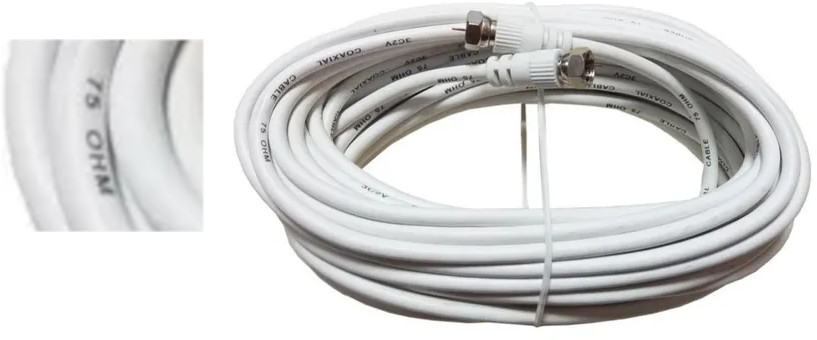
\includegraphics[height=6cm]{images/impedance.jpg}
\end{figure}
Dans un cable coaxial et pour une OPH, le courant et la tension sont proportionnels.
\subsubsection{Lien entre courant et tension}
\formule{Impédance caractéristique}
[
    Pour une OPH.
]
{
    $$u=\pm\footnote{+ pour une OPH dans le sens des $x$ croissants, - pour une OPH dans le sens de $x$ décroissants.} Z_c i$$
}
[
    \begin{itemize}
        \item $u$ la tension (en \unit{V})
        \item $i$ le courant (en \unit{A})
        \item $Z_c=\sqrt{\frac{\Lambda}{\Gamma}}$ l'impédance caractéristique (en \unit{\ohm})
    \end{itemize}
][o][o]
\flashcard{Impédance caractéristique d'un cable coaxial}{$Z_c=\sqrt{\frac{\Lambda}{\Gamma}}$}
\flashcard{Condition pour avoir $u=Z_ci$ dans un cable coaxial}{OPH qui se propage dans le sens croissant.}
\colle{Définir l'impédance caractéristique d'un cable coaxial. Établir le lien entre tension et courant pour des OPH se propageant dans le sens croissant et décroissant.}

\subsubsection{Réflexion sur une impédance terminale}
Lorsqu'une OPH incidente se réfléchit sur une impédance terminale, l'amplitude de l'onde réfléchie dépend de cette impédance terminale et de l'impédance caractéristique du cable.

\schema{Cable coaxial fermé sur une impédance terminale}{4cm}

\formule{Coefficient de réflextion sur une impédance terminale}
[
    \begin{itemize}
        \item L'onde incidente est une OPH : $u_i=u_{i,0}\cos(\omega_i t-k_ix)$.
        \item L'onde réfléchie est une OPH : $u_r=u_{r,0}\cos(\omega_r t+k_rx+\phi)$.
        \item Le cable est fermé sur une résistance $R$ en $x=0$.
    \end{itemize}
]
{
    $$\frac{u_{r,0}}{u_{i,0}}=\frac{R-Z_c}{R+Z_c}$$
}
[
    \begin{itemize}
        \item $u_{r,0}$ l'amplitude de l'onde réfléchie (en \unit{V})
        \item $u_{i,0}$ l'amplitude de l'onde incidente (en \unit{V})
        \item $R$ la résistance terminale (en \unit{\ohm})
        \item $Z_c$ l'impédance caractéristique du cable (en \unit{\ohm})
    \end{itemize}
][][o]

Lorsque l'impédance terminale est égale à l'impédance caractéristique du cable, il n'y a pas d'onde réfléchie.

\exemple{Cette propriété est utilisée dans les téléviseurs : la prise d'antenne est connectée à une résistance égale à l'impedance caractéristique du cable d'antenne afin qu'il n'y ait pas de réflexion dans le cable d'antenne.}
\colle{Montrer que l'onde réfléchie est nulle lorsqu'un cable coaxial est fermé sur une résistance égale à l'impédance caractéristique. Citer une application de cette propriété.}

\subsection{Impédance acoustique}
Par analogie avec le cable coaxial, on définit une impédance caractéristique.
\formule{Impédance acoustique}
[
    \begin{itemize}
        \item Pour une OPPH.
        \item Dans l'approximation acoustique.
        \item Le fluide est macroscopiquement au repos.
        \item L'évolution est adiabatique réversible.
    \end{itemize}
]
{
    $$P_1=Z_a \vv{v}.\vv{n}$$
}
[
    \begin{itemize}
        \item $P_1$ le champ de surpression (en \unit{Pa})
        \item $\vv{v}$ le champ de vitesse (en \unit{m.s^{-1}})
        \item $\vv{n}$ est un vecteur unitaire de même sens et direction que la propagation de l'onde (sans unité)
        \item $Z_a=\mu_0 c$ l'impédance acoustique (en \unit{Pa.s.m^{-1}})
    \end{itemize}
][o][o]
\flashcard{Impédance acoustique}{$Z_a=\mu_0 c$}
\flashcard{A quelle consition $P_1=Z_a v$ ?}{Pour une OPPH dans le sens croissant.}
\colle{Définir l'impédance acoustique. Établir le lien entre surpression et vitesse pour une OPH dans le sens croissant.}

\subsection{Relation de structure}
L'équation de Maxwell-Faraday fournit une relation entre les champs électrique et magnétique pour une OPPH.
\formule{Relation de structure}
[
    \begin{itemize}
        \item Pour une OPPH.
        \item Dans le vide.
    \end{itemize}
]
{
    $$\vv{B}=\frac{\vv{k}\wedge\vv{E}}{\omega}$$
}
[
    \begin{itemize}
        \item $\vv{B}$ le champ magnétique (en \unit{T})
        \item $\vv{k}$ le vecteur d'onde (en \unit{rad.m^{-1}})
        \item $\vv{E}$ le champ électrique (en \unit{V.m^{-1}})
        \item $\omega$ la pulsation (en \unit{rad.s^{-1}})
    \end{itemize}
][o][o]

Les vecteur $\vv{k}$, $\vv{E}$ et $\vv{B}$ sont mutuellement orthogonaux. De plus, le triplet $(\vv{k},\vv{E},\vv{B})$ est un trièdre direct.

\flashcard{Relation de structure}{$$\vv{B}=\frac{\vv{k}\wedge\vv{E}}{\omega}$$}
\colle{Démontrer la relation de structure pour une OPPH électromagnétique. En déduire que $(\vv{k},\vv{E},\vv{B})$ est un trièdre direct.}

\section{Aspectes énergétiques}
\subsection{Énergie acoustique}
Comme toute onde, les ondes acoustiques peuvent transporter de l'énergie.
\subsubsection{Vecteur de Poynting}
Le vecteur de Poynting est le vecteur densité volumique de courant d'énergie transportée par l'onde, c'est-à-dire la puissance surfacique que transporte l'onde.
\formule{Vecteur de Poynting}
[]
{
    $$\vv{\Pi}=P_1\vv{v}$$
}
[
    \begin{itemize}
        \item $\vv{\Pi}$ le vecteur de Poynting (\unit{W.m^{-2}})
        \item $P_1$ la surpression (en \unit{Pa})
        \item $\vv{v}$ le champ de vitesse (en \unit{m.s^{-1}})
    \end{itemize}
][o][o]
\flashcard{Vecteur de Poynting acoustique}{$$\Pi=P_i\vv{v}$$}

\subsubsection{Intensité acoustique}
L'intensité acoustique ou intensité sonore est la valeur moyenne de la norme du vecteur de Poynting.
\formule{Intensité acoustique}
[]
{
    $$I=\left<\|\vv{\Pi}\|\right>$$
}
[
    \begin{itemize}
        \item $I$ l'intensité acoustique (en \unit{W.m^{-2}})
        \item $\vv{\Pi}$ le vecteur de Poynting (\unit{W.m^{-2}})
    \end{itemize}
][o]
\flashcard{Intensité acoustique}{$$I=\left<\|\Pi\|\right>$$}
Les valeurs usuelles de l'intensité sonore s'étendent sur plusieurs ordres de grandeurs, on introduit donc le niveau sonore.
\formule{Niveau sonore}
[]
{
    $$I_{dB}=10\log{\frac{I}{I_0}}$$
}
[
    \begin{itemize}
        \item $I$ l'intensité acoustique (en \unit{W.m^{-2}})
        \item $I_0=\SI{1e-12}{W.m^{-2}}$ l'intensité acoustique de référence
    \end{itemize}
][o]
\flashcard{Niveau sonore}{$$I_{dB}=10\log{\frac{I}{I_0}}$$}
L'intensité acoustique de référence $I_0$ est le plus faible son discernable par l'oreille humaine.

\exemple{Quelques ordres de grandeur de niveaux sonores :
\begin{itemize}
    \item Pièce calme : \SI{20}{dB}
    \item Conversation à \SI{1}{m} : \SI{60}{dB}
    \item Rue animée (déclenchement du réflexe stapédien\footnote{Le réflexe stapédien est l'activation d'un muscle qui protège l'oreille interne. Ce muscle peut fatiguer, il est donc recommandé de ne pas avoir une exposition prolongée à ce niveau sonore.}) : \SI{80}{dB}
    \item Avion à quelques mètres (seuil de douleur) : \SI{120}{dB}
\end{itemize}}
\colle{Établir l'expression du vecteur de Poynting acoustique. Définir l'intensité acoustique et le niveau sonore. Citer quelques ordres de grandeur de niveaux sonores.}

\subsubsection{Retour sur les hypothèses de l'approximation acoustique}
Les niveaux sonores courants permettent de revenir sur les hypothèses de l'approximation acoustique pour les vérifier.
\formule{Hypothèses de l'approximation acoustique}
[
    \begin{itemize}
        \item Pour un OPPH.
        \item Dans l'air à la température de référence ($D_\text{th} = \SI{2e-5}{m^2.s^{-1}}$).
    \end{itemize}
]
{
    L'évolution est adiabatique.\\
    $$P_1\ll P_0$$
    $$\|\vv{v}\|\ll c$$
}[][][o]
\colle{En utilisant des ordres de grandeur de niveaux sonores usuels, vérifier que les hypothèses de l'approximation acoustique sont bien vérifiées.}
\subsubsection{Forme d'une onde sphérique}
Une onde sphérique est une onde dont les surfaces d'onde sont des sphères. Une onde sphérique dépend de la seule variable d'espace $r$.
\formule{Forme d'une onde sphérique}
[
    L'onde est sphérique.
]
{
    $$P_1=\frac{f(r-ct)}{r}+\frac{g(r+ct)}{r}$$
}
[
    \begin{itemize}
        \item $P_1$ la surpression (en \unit{Pa})
        \item $f$ et $g$ des fonctions quelconques
    \end{itemize}
][o]
\flashcard{Onde sphérique}{$$P_1=\frac{f(r-ct)}{r}+\frac{g(r+ct)}{r}$$}
Une onde sphérique s'atténue lors de sa propagation. La puissance de l'onde s'étale sur une surface de plus en plus large.

\application{Montrer que la puissance moyenne traverçant une sphère de rayon $r\gg\frac{1}{k}$ ne dépend pas de $r$.}

\subsection{Énergie électromagnétique}
\subsubsection{Conservation de l'énergie}
Le vecteur de Poynting désigne le vecteur densité de courant d'énergie électromagnétique.
\formule{Équation locale de conservation de l'énergie}
[
    L'onde peut communiquer de la puissance à des porteurs de charge.
]
{
    $$\frac{\partial w}{\partial t}=-\divv\vv{\Pi} - \vv{j_\text{élec}}.\vv{E}$$
}
[
    \begin{itemize}
        \item $w$ la densité volumique d'énergie électromagnétique (en \unit{J.m^{-3}})
        \item $\vv{\Pi}$ le vecteur de Poynting électromagnétique (en \unit{W.m^{-2}})
        \item $\vv{j_\text{élec}}$ le vecteur densité de courant électrique (en \unit{A.m^{-2}})
        \item $\vv{E}$ le champ électrique (en \unit{V})
    \end{itemize}
][][o]

Ce bilan d'énergie permet de déterminer le vecteur de Poynting et la densité volumique d'énergie.

\formule{Expression du vecteur de Poynting et de la densité volumique d'énergie}
[
    L'onde peut communiquer de la puissance à des porteurs de charge.
]
{
    $$w=\frac{\epsilon_0E^2}{2}+\frac{B^2}{2\mu_0}$$
    $$\vv{\Pi}=\frac{\vv{E}\wedge\vv{B}}{\mu_0}$$
}
[
    \begin{itemize}
        \item $w$ la densité volumique d'énergie électromagnétique (en \unit{J.m^{-3}})
        \item $\vv{\Pi}$ le vecteur de Poynting électromagnétique (en \unit{W.m^{-2}})
        \item $\vv{E}$ le champ électrique (en \unit{V.m^{-1}})
        \item $\vv{B}$ le champ magnétique (en \unit{T})
        \item $\mu_0$ la perméabilité magnétique du vide (en \unit{H.m^{-1}})
        \item $\epsilon_0$ la permittivité diélectrique du vide (en \unit{F.m^{-1}})
    \end{itemize}
]
[o][o]
\flashcard{Densité volumique d'énergie électromagnétique}{$$w=\frac{\epsilon_0E^2}{2}+\frac{B^2}{2\mu_0}$$}
\flashcard{Vecteur de Poynting électromagnétique}{$$\vv{\Pi}=\frac{\vv{E}\wedge\vv{B}}{\mu_0}$$}
\colle{En effectuant un bilan local d'énergie, établir par identification l'expression du vecteur de Poynting et de la densité volumique d'énergie électromagnétiques.}

\subsubsection{Flux de photons}
Un photon est une particule élémentaire sans masse qui transporte l'énergie des ondes électromagnétiques.

\formule{Relation de Planck-Einstein}
[]
{$$\mathcal{E}=h\nu$$}
[
    \begin{itemize}
        \item $\mathcal{E}$ l'énergie d'un photon (en \unit{J})
        \item $h\approx\SI{6.63e-34}{J.s}$ la constante de Plank
        \item $\nu$ la fréquence de l'onde (en \unit{Hz})
    \end{itemize}
][o]
\flashcard{Relation de Plank-Einstein}{$$\mathcal{E}=h\nu$$}

\application{Déterminer le débit de photons d'un pointeur laser rouge de puissance \SI{5}{mW}.}

\subsubsection{Énergie d'une OPPH}
\formule{Densité volumique d'énergie d'une OPPH}
[
    \begin{itemize}
        \item Dans le vide.
        \item L'onde est une OPPH : $\vv{E}=E_0\cos(\omega t-kx)\vv{e_y}$
    \end{itemize}
]
{
    $$\left< w\right>=\frac{\epsilon_0 E_0^2}{2}$$
}
[
    \begin{itemize}
        \item $w$ la densité volumique d'énergie électromagnétique (en \unit{J.m^{-3}})
        \item $E_0$ l'amplitude de l'onde (en \unit{V.m^{-1}})
        \item $\epsilon_0$ la permittivité diélectrique du vide (en \unit{F.m^{-1}})
    \end{itemize}
][][o]

Pour une OPPH, l'énergie est équirépartie entre la forme magnétique et la forme électrique.

\formule{Vecteur de Poynting}
[
    \begin{itemize}
        \item Dans le vide.
        \item L'onde est une OPPH : $\vv{E}=E_0\cos(\omega t-kx)\vv{e_y}$
    \end{itemize}
]
{
    $$\left<\vv{\Pi}\right>=\frac{E_0^2}{2c\mu_0}\vv{e_x}$$
}
[
    \begin{itemize}
        \item $\vv{\Pi}$ le vecteur de Poynting électromagnétique (en \unit{W.m^{-2}})
        \item $E_0$ l'amplitude de l'onde (en \unit{V.m^{-1}})
        \item $\mu_0$ la perméabilité magnétique du vide (en \unit{H.m^{-1}})
        \item $c$ la célérité de la lumière dans le vide (en \unit{m.s^{-1}})
    \end{itemize}
][][o]

La direction de propagation de l'énergie est la même que la direction de propagation de l'onde.